\begin{defi}{Polynômes de \textsc{Tchebychev}}
    Les polynômes de \textsc{Tchebychev} de première espèce sont les uniques polynômes $(\Tcheby_n)_{n \geqslant 0}$ définis sur $]-1, 1[$ par
    $$\forall \theta \in \R,\ \Tcheby_n (\cos \theta) = \cos(n \theta).$$
\end{defi}

Vérifions tout d'abord qu'une telle suite existe bien et qu'elle est unique.

\begin{marginfigure}[-4.5cm]
    \centering
	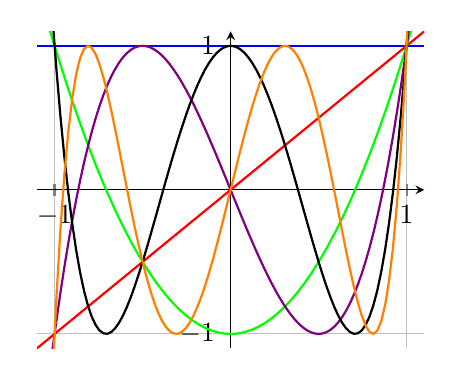
\begin{tikzpicture}
    \begin{axis}[width=6.5cm,
        axis lines=middle,
        grid=major,
        xmin=-1.1, xmax=1.1,
        ymin=-1.1, ymax=1.1,
        % xlabel=$x$, xlabel style={right},
        % ylabel=$y$, ylabel style={above},
        tick style={thick},
        ticklabel style={font=\normalsize},
        xtick={-1, 0, 1}, 
        ytick={-1, 0, 1},
        % legend entries={0.5x},
            legend style={
            at={(1.05,0.4)},
            anchor=north,
            legend columns=1},
            legend cell align={left}
    ]
    
    \def\a{-1.1}
    \def\b{1.1}
    
    \addplot[blue,thick,samples=100,domain=\a:\b] {1};
    \addplot[red,thick,samples=100,domain=\a:\b] {x};
    \addplot[green,thick,samples=100,domain=\a:\b] {2*x^2-1};
    \addplot[violet,thick,samples=100,domain=\a:\b] {4*x^3-3*x};
    \addplot[black,thick,samples=100,domain=\a:\b] {8*x^4-8*x^2+1};
    \addplot[orange,thick,samples=100,domain=\a:\b] {16*x^5-20*x^3+5*x};
    
   % \legend{$\Leg_0$, 
   %         $\Leg_1$,
%            $\Leg_2$,
%            $\Leg_3$,
 %           $\Leg_4$,
  %          $\Leg_5$
   %         }
    \end{axis}
\end{tikzpicture}
	\caption*{\centering Polynômes de \textsc{Tchebychev} de première espèce}
	\begin{align*}
	   	\color{blue} \Tcheby_0 = 1 \\
    	\color{red} \Tcheby_1 = x \\
    	\color{green} \Tcheby_2 = 2x^2-1 \\
    	\color{purple} \Tcheby_3 = 4x^3-3x \\
    	\color{black} \Tcheby_4 = 8x^4-8x^2+1 \\
    	\color{orange} \Tcheby_5 = 16x^5-20x^3+5x
	\end{align*}
\end{marginfigure}

\begin{preuve}
    \begin{description}
        \item[Existence] Nous allons montrer que la suite $(\Tcheby_n)_{n \geqslant 0}$ vérifie une relation de récurrence. \\
        Soit $n \in \N$,
        \begin{align*}
            \Tcheby_{n+2}(\cos \theta) &= \cos((n+2) \theta) \\
            &= \cos((n+1) \theta) \cos(\theta) - \sin((n+1) \theta) \sin(\theta) \\
            &= \Tcheby_{n+1}(\cos \theta) \cos(\theta) - \frac{1}{2} \left(\cos(n \theta) - \cos((n+2)\theta)\right) \\
            \Tcheby_{n+2}(\cos \theta) &= \Tcheby_{n+1}(\cos \theta) \cos(\theta) - \frac{1}{2} \Tcheby_n(\cos \theta) + \frac{1}{2} \Tcheby_{n+2}(\cos \theta)
        \end{align*}
        d'où
        $$\Tcheby_{n+2} = 2X \Tcheby_{n+1} - \Tcheby_n.$$
        \item[Unicité] L'unicité de $\Tcheby_n$ pour $n$ fixé est garantie pas l'identification de \ptnclegras{deux polynômes coïncidant} sur $]-1, 1[$. 
    \end{description}
\end{preuve}

\marginnote[-6cm]{
    \begin{kaobox}[frametitle=Formule de trigonométrie]
        $$\sin a \sin b = \frac{1}{2} \big( \cos(a-b) - \cos(a+b) \big)$$
    \end{kaobox}
}

\begin{exercice}
    Soit $n \in \N$, déterminer une expression de $\Tcheby_n$.
\end{exercice}  

\begin{solution}
    \begin{align*}
        \cos(n \theta) &= \Reel \left( \me^{\mi n \theta}) = \Reel((\cos \theta + \mi \sin \theta)^n \right)\\
        &= \Reel\left( \sum_{k=0}^n \binom{n}{k} (\cos\theta)^k (\mi \sin\theta)^{n-k} \right) \\
        &= ...
    \end{align*}
    $$\forall n \in \N,\ \Tcheby_n = \sum_{k=0}^{\lfloor n / 2 \rfloor} (-1)^k \binom{n}{2k} X^{n-2k} (1-X^2)^k.$$
\end{solution}

\begin{prop}{}
    \begin{enumerate}
        \item $$\deg \Tcheby_n = n \text{ et } \mathrm{cd}\, \Tcheby_n = 2^{n-1}$$
        \item $\Tcheby_n$ est pair si $n$ est pair et vice versa. \\
        \item Pour tout $n, m$, $\Tcheby_n \circ \Tcheby_m = \Tcheby_{nm}$. \\
        \item $$(1-x^2) \Tcheby''_n(x) - x \Tcheby'_n(x) + n^2 \Tcheby_n(x) = 0.$$
        \item $\Tcheby_n$ admet $n$ racines simples qui sont
        $$a_{k,n} = \cos \left( \frac{(2k-1) \pi}{2n}\right),\ k \in \llbracket 1, n \rrbracket.$$
        \item Sur $[-1, 1]$, $\Tcheby_n$ admet $n+1$ extrema égaux à $1$ en les points
        $$b_{k,n} = \cos\left( \frac{k \pi}{n} \right),\ k \in \llbracket 0, n \rrbracket.$$
    \end{enumerate}
\end{prop}

\begin{preuve}
    \begin{enumerate}
        \item ff
        \item ff
        \item 
    \end{enumerate}
\end{preuve}

